%!LW recipe=latexmk (latexmkrc)
% The above line tells which recipe LaTeX Workshop shall use to build the file.
% See https://github.com/James-Yu/LaTeX-Workshop/wiki/Compile#latex-recipes
\documentclass[12pt]{article}

\usepackage{sbc-template}
\usepackage{graphicx,url}
\usepackage[utf8]{inputenc}
\usepackage[english]{babel}


\sloppy

\title{Practical Challenges in Reproducing Large-Scale Code Retrieval Benchmarks: The XCodeEval Experience}

\author{Henrique Krausbug Correa\inst{1}, Viviane Pereira Moreira\inst{1}, Dennis Giovani Balreira\inst{1}}


\address{Instituto de Informática -- Universidade Federal do Rio Grande do Sul
  (UFRGS)\\
  Caixa Postal 15.064 -- 91.501-970 -- Porto Alegre -- RS -- Brazil
  \email{\{henrique,viviane,dgbalreira\}@inf.ufrgs.br}
}

\begin{document} 

\maketitle


% ( 150 words approximately )
\begin{abstract}
  This paper investigates the reproducibility of the XCodeEval NL-Code retrieval benchmark, with a focus on understanding the notably lower retrieval accuracy for the D programming language compared to other languages. We aimed to replicate the original experimental setup using Dense Passage Retrieval (DPR) with StarEncoder, following the official methodology and dataset splits. Despite substantial engineering effort and incremental optimizations, the experiment was ultimately constrained by resource and platform limitations, particularly during the embedding generation phase for the full 25 million-document corpus. Alternative approaches, such as TF-IDF baselines, were found infeasible due to scalability and hardware constraints. Our experience highlights the critical importance of robust infrastructure, scalable algorithms, and transparent reporting in large-scale NLP research. We discuss the challenges encountered, lessons learned, and recommendations for future work, emphasizing the need for improved institutional support and methodological innovation to enable reproducible benchmarking in academic research.
\end{abstract}
     
\begin{resumo} 
  Este artigo investiga a reprodutibilidade do benchmark XCodeEval para recuperação NL-Code, com foco em compreender a precisão notavelmente inferior da recuperação para a linguagem de programação D em comparação com outras linguagens. Nosso objetivo foi replicar a configuração experimental original utilizando Dense Passage Retrieval (DPR) com StarEncoder, seguindo a metodologia oficial e as divisões do conjunto de dados. Apesar de um esforço significativo de engenharia e de otimizações incrementais, o experimento foi, em última instância, limitado por restrições de recursos e de plataforma, especialmente durante a fase de geração de embeddings para o corpus completo de 25 milhões de documentos. Abordagens alternativas, como os baselines baseados em TF-IDF, mostraram-se inviáveis devido a limitações de escalabilidade e hardware. Nossa experiência destaca a importância crítica de uma infraestrutura robusta, algoritmos escaláveis e relatórios transparentes na pesquisa em PLN em larga escala. Discutimos os desafios enfrentados, as lições aprendidas e recomendações para trabalhos futuros, enfatizando a necessidade de maior apoio institucional e inovação metodológica para viabilizar benchmarks reproduzíveis na pesquisa acadêmica.
\end{resumo}

\section{Introduction}
% (1 page)

% Context: Why is code retrieval important in NLP? What is XCodeEval’s role?

% Motivation:
%  - XCodeEval NL-Code task benchmark reports a great accuracy for all languages, but D language has a lower accuracy.
%  - Authors statement: "We suspect that the limited availability of resources for D in both The Stack (Kocetkov et al., 2022) dataset (training corpora of StarEncoder) and our XCODEEVAL dataset could account for this discrepancy. Also, the presence of more hard negative candidates (i.e., very similar to a correct code) makes it a challenging task to identify similar codes."
%  - However, by checking TABLE 4, D dataset size is greater than other languages such as Perl and Ocaml, which have higher accuracy. 

% Research questions:
%   - What is the root cause analysis for D language lower accuracy on code retrieval tasks?
%   - Can this performance be improved based on NLP class topics and published articles related to this topic?

Modern software development increasingly relies on AI-powered tools that combine code retrieval and generation capabilities to assist developers.
Recent systems like RepoCoder \cite{Zhang2023} demonstrate how iterative retrieval-generation pipelines can leverage repository-wide context for code completion.
This highlights the importance of precise code retrieval as a foundation for AI-assisted programming tools — from IDE autocompletion to documentation generation and code reuse recommendation systems \cite{Ziegler2022}.
However, to be effective, code retrieval systems must address two primary challenges:

\begin{itemize}
  \item \textbf{Semantic-Execution Gap}: Bridging the disparity between natural language intent (queries) and executable implementations (retrieval targets), requiring understanding of both functionality and syntax \cite{Wan2019}
  \item \textbf{Multilingual Context}: As shown in repository-level tools like RepoCoder, retrieval must handle cross-file dependencies and language-specific patterns while maintaining execution correctness
\end{itemize}

The XCodeEval benchmark \cite{Khan2023} formalizes these requirements through its NL-Code retrieval task over 25M coding examples from about 7.5K unique algorithmic problems. These tasks evaluate systems on their ability to match natural language problem descriptions with executable implementations across 17 programming languages. For evaluation and analysis, it uses the StarEncoder \cite{Li2023} architecture and computed the top-k retrieval accuracy for each of the 17 query languages. Table \ref{tab:xcodeeval-performance} summarizes the performance of StarEncoder on the XCodeEval benchmark for a subset of languages. Author's discussion of results is as follows:

\begin{quote}
\textit{``For NL-Code, performance is good across all languages except for D. We suspect that the limited availability of resources for D in both The Stack \cite{Kocetkov2022} dataset (training corpora of StarEncoder) and our XCodeEval dataset could account for this discrepancy. Also, the presence of more hard negative candidates (i.e., very similar to a correct code) makes it a challenging task to identify similar codes.''}~\cite{Khan2023}
\end{quote}

\begin{table}[ht]
\centering
\caption{Summary of performance of StarEncoder \cite{Li2023}
for k = 100 in ~\cite{Khan2023}}
\label{tab:xcodeeval-performance}
\begin{tabular}{lccccccc}
\hline
\textbf{Metric} & \textbf{C++} & \textbf{Java} & \textbf{Python} & \textbf{D} & \textbf{Perl} & \textbf{Ocaml} & \textbf{AVG.} \\
\hline
Acc@K & 83.81 & 84.72 & 84.57 & 68.98 & 81.33 & 85.45 & 83.83 \\
\hline
\end{tabular}
\end{table}

However, our analysis reveals a notable performance discrepancy in the XCodeEval benchmark: while the average top-100 retrieval accuracy across languages is 83.83\%, the D programming language achieves only 68.98\%. This is surprising given the data distribution shown in Table~\ref{tab:xcodeeval-selected}, which presents the three languages with the largest and smallest retrieval corpus sizes.

As shown, D has a larger training set and a greater corpus size than some better-performing languages such as Perl and Ocaml. In contrast, languages like C++ and Java have much larger corpora, yet D's retrieval accuracy is significantly lower than even languages with smaller datasets.

This contradicts the common assumption that dataset or corpus size is the primary determinant of retrieval performance. Instead, as echoed in repository-level studies~\cite{Zhang2023}, retrieval quality appears to depend more on the context relevance and characteristics of the data than on its quantity. This motivates a deeper investigation into the factors affecting D's performance.

\begin{table}[ht]
\centering
\caption{Retrieval statistics for selected languages in ~\cite{Khan2023}}
\label{tab:xcodeeval-selected}
\begin{tabular}{lrrr}
\hline
\textbf{Language} & \textbf{Train Size} & \textbf{Test Size} & \textbf{Corpus Size} \\
\hline
C++     & 6,181  & 1,098   & 18,212,508 \\
Java    & 5,930  & 1,021   & 2,523,044 \\
Python  & 4,930  & 859     & 2,290,854 \\
D       & 3,359  & 521     & 15,984 \\
Perl    & 1,276  & 412     & 11,035 \\
Ocaml   & 1,424  & 381     & 7,012 \\
\hline
\end{tabular}
\end{table}

We investigate:
\begin{itemize}
    \item What factors beyond dataset size contribute to D's lower retrieval performance?
    \item Is it possible to improve retrieval accuracy for low-resource languages through targeted NLP approaches?
\end{itemize}

This work aims to:
\begin{enumerate}
    \item Reproduce the XCodeEval NL-Code retrieval benchmark using the specified Dense Passage Retrieval (DPR) architecture with StarEncoder \cite{Li2023}
    \item Investigate whether standard NLP techniques for low-resource scenarios can improve results
\end{enumerate}

The remainder of this paper is structured as follows:
Section 2 covers background on code retrieval and the XCodeEval benchmark.
Section 3 reviews related work.
Section 4 details our methodology for benchmark reproduction.
Section 5 presents experimental results, and
Section 6 concludes with findings and future directions.

\section{Background}

% (1–2 pages)

% Terminilogy: Define key terms (e.g., code retrieval, dense passage retrieval).

% Dense Passage Retrieval (DPR): How it works, why it’s used for code retrieval.

\subsection{Code Retrieval}

Code retrieval is the process of searching and retrieving relevant code snippets or implementations based on user queries, which can be in natural language or code form. This task is crucial for various applications, including code completion, bug fixing, and documentation generation. The challenge lies in effectively matching user intent with the correct code implementations, especially across multiple programming languages ~\cite{Kim2021}.

The essential components of a code retrieval system are illustrated in Figure~\ref{fig:code-search-components} and summarized below:

\begin{figure}[ht]
\centering
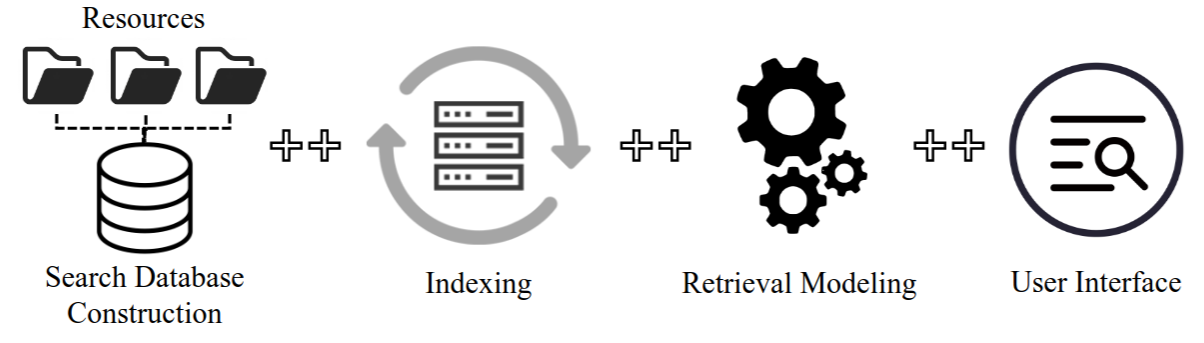
\includegraphics[width=0.7\textwidth]{images/code-search-components.png}
\caption{Basic Code Search Components from \cite{Kim2021}}
\label{fig:code-search-components}
\end{figure}

\begin{itemize}
    \item \textbf{Search Database}: Defines the source code repository or dataset from which code is retrieved. This may involve web crawlers to collect code files, API documentation, or Q\&A pairs. The search base can be structured as a relational database, file system, or plain text corpus, depending on the application.
    \item \textbf{Indexer}: Optimizes data access by building efficient data structures for retrieval. Common techniques include inverted indexing (mapping terms to document locations), as well as B+ trees, graph-based, or positional indexing, all aimed at speeding up code snippet retrieval.
    \item \textbf{Retrieval Model}: The core of the system, responsible for matching user queries to relevant code. Retrieval models can be based on text matching, matrix computations, or vector similarity measures, and are often the main differentiator between code search approaches.
    \item \textbf{User Interface}: Presents retrieval results to users, either through standalone search engines or integration with development environments (IDEs). The interface must accommodate diverse user needs and workflows.
\end{itemize}

\subsection{Dense Passage Retrieval (DPR)}

Dense Passage Retrieval (DPR)~\cite{Karpukhin2020} is a neural retrieval framework originally developed for open-domain question answering, but now widely adopted for code and document retrieval tasks. DPR is built on a bi-encoder architecture, where two separate encoders independently map queries and passages (or code snippets) into a shared dense vector space. This enables efficient retrieval by comparing vector representations using simple similarity measures, such as the dot product.

Figure~\ref{fig:dpr-architecture} illustrates the main workflow of DPR, which involves two stages:
\begin{itemize}
    \item \textbf{Indexing}: All candidate passages (or code snippets) are encoded into dense vectors using a passage encoder. These vectors are stored in an efficient similarity search index, such as FAISS~\cite{Johnson2017}, allowing for rapid retrieval even from very large collections.
    \item \textbf{Retrieval}: At query time, the input question or natural language description is encoded by a separate query encoder. The system then retrieves the top-$k$ passages whose vectors are most similar to the query vector.
\end{itemize}

\begin{figure}[ht]
\centering
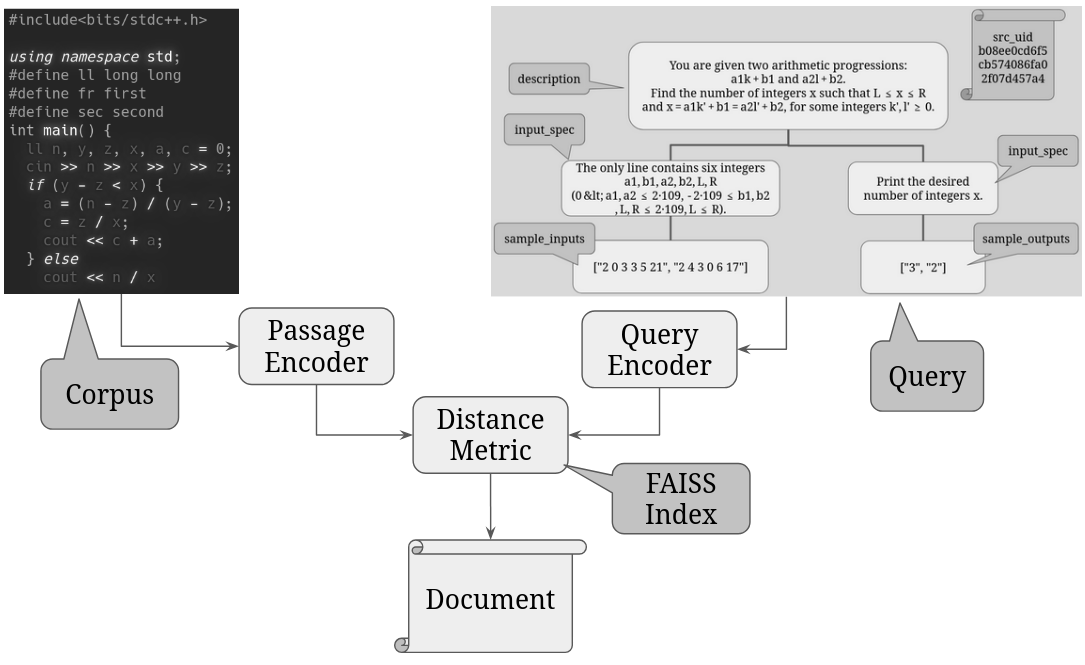
\includegraphics[width=1.0\textwidth]{images/dpr-architecture-gray.png}
\caption{DPR Architecture conceptual overview}
\label{fig:dpr-architecture}
\end{figure}

A key advantage of DPR is that both encoders are trained to maximize the similarity between relevant query-passage pairs while minimizing it for irrelevant pairs. The last technique is called in-batch negative sampling \cite{Choi2021}, where negative examples are drawn from the same batch during training.

For code retrieval, DPR's architecture is particularly effective because it can learn to bridge the gap between natural language queries and code implementations, even across multiple programming languages. By leveraging dense vector representations, DPR supports semantic search, enabling retrieval of relevant code snippets that may not share surface-level keywords with the query.

\section{Related Work}

% (1–2 pages)

% Post Work: Summarize key papers on code retrieval that cite XCodeEval and criticize its limitations.

COIR (Code Information Retrieval Benchmark)~\cite{Li2025} was introduced to address the limitations of existing code retrieval benchmarks by providing a broader, more diverse, and rigorous evaluation framework. Its main goal is to enable robust assessment of retrieval models across a wide range of tasks and domains. COIR integrates ten curated datasets, covering eight retrieval tasks (including text-to-code, code-to-code, and hybrid scenarios) across seven domains. This diversity is intended to reflect real-world code retrieval needs more accurately than previous benchmarks. COIR explicitly critiques XCodeEval for several reasons:
\begin{itemize}
    \item \textbf{Task Diversity:} XCodeEval, like other benchmarks, primarily focuses on a narrow set of retrieval tasks (e.g., natural language to code), which may not generalize to broader, real-world scenarios where queries and targets can be both code and text in various forms.
    \item \textbf{Domain Coverage:} XCodeEval's dataset is largely derived from programming contest challenges, limiting its applicability to other domains such as open-source projects, bug fixing, or code summarization.
    \item \textbf{Overfitting and Generalizability:} COIR notes that many models have overfitted to existing leaderboards, including XCodeEval, which can mask true retrieval performance and hinder progress.
    \item \textbf{Evaluation Consistency:} The lack of a standardized evaluation framework across benchmarks like XCodeEval complicates fair comparison and reproducibility.
\end{itemize}
  
\cite{Dehghan2024} provides a comprehensive literature review focused on evaluating the code reasoning capabilities of Large Language Models (LLMs). The main objective of this work is to analyze existing benchmarks and evaluation frameworks, identifying their effectiveness in assessing deeper aspects of code understanding—such as semantic comprehension, execution behavior, and reasoning about program logic—beyond mere code generation. The review highlights the need for more robust, unbiased, and contamination-resistant benchmarks that can accurately measure an LLM's ability to reason about code across multiple languages and real-world scenarios. \cite{Dehghan2024} discusses XCodeEval as a significant execution-based, multilingual benchmark for code-related LLM evaluation. The review acknowledges XCodeEval's strengths, such as its large scale, multilingual coverage, and use of execution-based metrics. However, it also points out several limitations:
\begin{itemize}
    \item \textbf{Domain Diversity:} XCodeEval's data is sourced exclusively from codeforces.com, limiting the diversity of coding styles and problem domains.
    \item \textbf{Resource Discrepancies:} There are notable imbalances in the number of samples per programming language, which can bias evaluation results.
    \item \textbf{Lack of Modularity:} The benchmark primarily contains document-level, non-modular code, which may not reflect real-world software engineering practices.
    \item \textbf{Real-World Coverage:} XCodeEval may not fully capture the complexity of real-world coding challenges, such as those involving external systems or edge cases.
\end{itemize}

These considerations reinforce the need for more comprehensive and representative benchmarks, supporting the motivation for our analysis of retrieval performance in multilingual code tasks.
generalizability

\section{Methodology}

%  (2–3 pages)

% Describe your approach to reproducing the XCodeEval benchmark.

% XCodeEval Benchmark: Tasks, dataset structure, and original paper’s setup.

% Data Preparation: How you processed XCodeEval (NL-Code template, corpus format).

% Model Setup:

%   DPR architecture (query/corpus encoders, multilingual training).

%   Hyperparameter (batch size, seq length, epochs) from the original paper.

% Evaluation Plan: Top-*k* accuracy (*k*=100), corpus/query embedding generation.

In this section, we describe our approach to reproducing the XCodeEval NL-Code retrieval benchmark, including a detailed overview of the task definition, dataset structure, and the original experimental setup as described in~\cite{Khan2023}.

\subsection{Dataset Overview}

The XCodeEval benchmark~\cite{Khan2023} is designed to evaluate the ability of models to retrieve relevant and executable code based on natural language (NL) problem descriptions. Specifically, the NL-Code retrieval task requires the system to match a given problem statement in natural language to the most relevant and correct code implementation from a large pool of candidate solutions. Retrieved code is considered correct only if it passes all associated unit tests for the given problem, ensuring that the retrieval process is not only semantically accurate but also functionally correct. Dataset is constructed from over 25 million code samples collected from codeforces.com, covering 7,514 unique algorithmic problems and 17 programming languages. For the NL-Code retrieval task, each instance consists of:
\begin{itemize}
    \item \textbf{nl}: The natural language problem description, including input and output specifications.
    \item \textbf{positive\_code}: A list of code solutions that correctly solve the problem (i.e., pass all unit tests).
    \item \textbf{negative\_code}: A list of code solutions that are incorrect or buggy for the problem.
    \item \textbf{src\_uid}: A unique identifier linking the code to its associated problem.
    \item \textbf{file\_name}: The source file from which the data instance was loaded.
\end{itemize}

Figure~\ref{fig:training} provides a visual summary of these dataset attributes, illustrating how each training instance pairs a problem description with both positive and negative code examples. This structure enables the use of contrastive learning approaches, where the model learns to distinguish correct solutions from hard negatives.

\begin{figure}[ht]
\centering
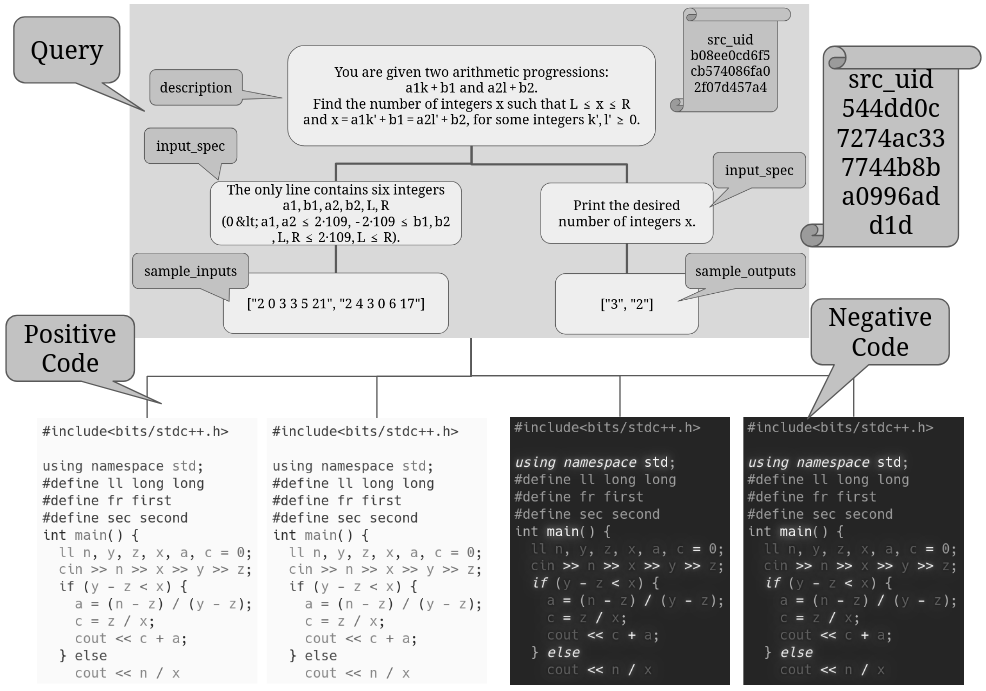
\includegraphics[width=1.0\textwidth]{images/task-gray.png}
\caption{Training dataset sample with query, positive and negative code}
\label{fig:training}
\end{figure}

\subsection{Reference Paper Setup}

The original XCodeEval paper employs a bi-encoder architecture based on Dense Passage Retrieval (DPR)~\cite{Karpukhin2020}, using StarEncoder~\cite{Li2023} as the backbone for both the query (NL) and code encoders. The model is trained in a multilingual manner, leveraging all available languages in the dataset. Training is performed with a maximum sequence length of 1024 tokens, an effective batch size of 48, and for 37 epochs. During training, in-batch negative sampling is used, where negative examples are drawn from other instances in the same batch.

For evaluation, the model encodes all candidate code snippets in the retrieval corpus into dense vectors. At query time, the natural language description is encoded, and the system retrieves the top-$k$ most similar code vectors using a similarity search (e.g., dot product). Retrieval accuracy@k is then computed as the proportion of queries for which a correct code is found within the top-$k$ results.

\subsection{Data Preparation}

To ensure fidelity with the original XCodeEval benchmark \cite{Khan2023}, we used the NL-Code template as provided, without any modifications or filtering of examples. Tokenization and input formatting were performed using the HuggingFace Transformers pipeline \cite{Wolf2020}, specifically employing the same tokenizer configuration as the original StarEncoder model \cite{Li2023}. No filtering or modification of examples was applied. All code and natural language inputs were tokenized with a maximum sequence length of 1024 and padded as needed, matching the original XCodeEval setup. All available programming languages in the dataset were included to maintain comparability with the original results. The default train, validation, and test splits provided by XCodeEval were used throughout. The source code for all data preparation and experimental procedures described in this paper is publicly available at \url{https://github.com/henrikcorrea/nlp-tf}.

\subsection{Model Setup}

For model implementation, we relied on the HuggingFace Transformers library. We used the official StarEncoder and Dense Passage Retrieval (DPR) models \cite{Karpukhin2020} without any architectural changes or custom modifications. Positive and negative samples were used as provided in the dataset, with no additional sampling or augmentation, in order to faithfully reproduce the original XCodeEval results.

\subsection{Evaluation}

Retrieval accuracy@k was computed using the same retrieval corpus and evaluation methodology as the original XCodeEval paper. No post-processing or filtering was applied to the retrieved results. The value of $k$ was set to match the original benchmark (e.g., $k=100$), and the evaluation strictly followed the official test split and metrics.

\subsection{Environment}

All experiments were executed on a cloud GPU environment provided by RunPod (\url{https://www.runpod.io/}), specifically using a pod with 4x RTX A4000 GPUs (64 GB total VRAM), 248 GB RAM, 56 vCPUs, and 400 GB NVMe storage. While several implementation challenges were encountered, these are discussed in detail in the Experimental Results section.

\section{Experimental Results}

% (3–4 pages)

% Describe framework, tools retrieval task results, and any preliminary findings.

% Expected vs. Actual: Compare original paper’s metrics to your observations.

% Possible Reasons for Divergence:

%   Training time insufficient? Hyperparameters not optimized?

%   Data preprocessing differences (e.g., template formatting).

% Qualitative Examples: Show some query-corpus pairs (even if not evaluated fully).

Despite extensive efforts to reproduce the XCodeEval NL-Code retrieval benchmark, our experiments were ultimately constrained by resource and platform limitations. This section details the experimental framework, encountered bottlenecks, and key lessons learned.

\subsection{Framework and Tools}

All experiments were conducted using the HuggingFace Transformers library, PyTorch, and the official StarEncoder model, following the methodology described in Section~4. The data pipeline and embedding generation were implemented in Python, leveraging GPU acceleration where possible. Experiments were executed on RunPod cloud instances with up to 4x RTX A4000 GPUs, 248 GB RAM, and 400 GB NVMe storage.

\subsection{Data Preparation Bottlenecks}

The primary bottleneck occurred during the embedding generation phase for the 25M-document corpus. Several rounds of optimization were required to improve throughput:
\begin{itemize}
    \item \textbf{Single GPU, no optimization:} 40 documents/second.
    \item \textbf{PyTorch DataParallel (2x GPUs):} 70 documents/second.
    \item \textbf{Reduced precision (bfloat16):} 200 documents/second.
    \item \textbf{ProcessPoolExecutor (4x GPUs):} 520 documents/second.
\end{itemize}
Despite these improvements, further progress was hindered by RAM and storage issues. The HuggingFace \texttt{datasets.map()} operation incrementally increased memory and disk usage, eventually exceeding available resources. Additionally, RunPod platform constraints prevented dynamic resource scaling or intervention during long-running jobs.

These optimizations were achieved through a combination of leveraging multiple GPUs, reducing numerical precision, and parallelizing the workload at the process level. Each step required significant code refactoring and experimentation with PyTorch and Python concurrency tools. However, even with these improvements, the process remained highly resource-intensive.

A major challenge was the management of RAM and storage during embedding generation. The HuggingFace \texttt{datasets.map()} operation, used to apply the embedding function across the dataset, incrementally increased both memory and disk usage. This was due to the internal caching and temporary storage mechanisms of the library, which are not easily configurable or optimized for extreme-scale datasets. As a result, the process would eventually exceed available RAM or disk space, causing the job to fail.

\subsection{Resource Management and Platform Limitations}

Resource usage was monitored via \texttt{htop} (CPU/RAM), alongside RunPod dashboard (GPU/disk). However, memory and storage spikes often became apparent only after significant runtime, at which point mitigation was impossible without restarting the job and losing progress. 

Additionally, on RunPod, it was not possible to dynamically scale resources or adjust hardware specifications during a running job. If a memory or storage bottleneck was detected mid-process, the only option was to terminate and restart the pod, losing all progress. Machine availability was also inconsistent, sometimes delaying experimentation. Nevertheless, RunPod's competitive pricing made it attractive for large-scale experiments compared to other cloud providers.

\subsection{Partial Results and Trade-offs}

Pipeline validation was performed on small data subsets (e.g., using \texttt{dataset.select(n)}), confirming the technical correctness of the approach. However, no partial or downsampled results are reported here, as reducing the corpus size would invalidate the comparability of retrieval accuracy across languages—a key focus of this study.

Specifically, the central motivation of this work is to analyze retrieval performance discrepancies between languages under the same experimental conditions as the original XCodeEval benchmark. Using a reduced corpus would introduce artificial biases: for example, some languages might benefit disproportionately from a smaller dataset, while others could see their performance degraded, distorting the original distribution and making it impossible to draw meaningful conclusions about the causes of observed accuracy gaps. Furthermore, any improvements or degradations observed on a downsampled corpus would not necessarily generalize to the full-scale benchmark, undermining the validity of the analysis. For these reasons, all reported results and conclusions are restricted to the full dataset setting, in line with the original benchmark protocol.

\subsection{Alternative Approaches}

Sparse retrieval baselines, such as TF-IDF \cite{Ramos2003} implemented via scikit-learn (\url{https://scikit-learn.org}), were considered as a fallback to provide at least a baseline for comparison. However, several critical limitations made this approach infeasible for the XCodeEval corpus:

\begin{itemize}
    \item \textbf{Single-CPU Limitation:} The standard scikit-learn TF-IDF implementation only supports single-CPU processing. There is no straightforward way to parallelize or distribute the computation across multiple CPUs or GPUs within the library, which severely limits throughput for very large datasets.
    \item \textbf{Vocabulary Fitting Requirement:} TF-IDF requires fitting the entire vocabulary from the corpus before any transformation can occur. For the XCodeEval dataset, this means processing all 25 million documents in memory to build the vocabulary and compute term statistics, which is both memory- and time-intensive.
    \item \textbf{Scalability Constraints:} Given these limitations, a full TF-IDF embedding computation for the entire corpus was estimated to take over 21 days on the available hardware, compared to approximately 12 hours for the DPR pipeline (if resources were sufficient). The lack of GPU support and distributed processing options for TF-IDF further exacerbated the scalability challenge.
\end{itemize}

Due to these factors, it was not feasible to generate a TF-IDF baseline for this study. This highlights a broader challenge in applying traditional sparse retrieval methods to modern, large-scale code retrieval benchmarks, and underscores the importance of scalable, GPU-accelerated solutions for current NLP research.

\subsection{Reproducibility and Documentation}

All steps, code, and encountered issues were documented in Jupyter notebooks and version-controlled via GitHub (\url{https://github.com/henrikcorrea/nlp-tf}). While the original StarEncoder checkpoint lacked detailed documentation, all dataset and pipeline questions were resolved independently.

\subsection{Lessons Learned}

This work highlights several practical lessons for large-scale NLP experiments:
\begin{itemize}
    \item Start with affordable, previous-generation GPUs to build expertise before scaling up.
    \item Ensure code is robust to failures and supports progressive checkpointing, especially for long-running cloud jobs.
    \item Plan for significant storage overhead during data processing, particularly with frameworks like HuggingFace Datasets.
    \item Institutional support for GPU clusters with adequate storage is essential for reproducible research in modern NLP.
\end{itemize}

Despite not achieving full reproduction of the XCodeEval benchmark, the project provided valuable insights into the practical challenges of large-scale code retrieval research and the importance of infrastructure in enabling reproducible results.


\section{Conclusion}

% (0.5 page)

% Lessons Learned: What would you do differently with more time/resources?

% Summary of efforts, challenges, and open questions.

% Alternative Approaches: Smaller models (e.g., ColBERT), approximate nearest-neighbor search (FAISS).

% Broader Implications: Reproducibility challenges in NLP research.

This work set out to reproduce the XCodeEval NL-Code retrieval benchmark and investigate the factors underlying the D programming language's lower retrieval accuracy. Despite significant engineering effort and incremental optimizations, the experiment was ultimately constrained by resource and platform limitations, particularly during the embedding generation phase for the full 25M-document corpus.

Several key lessons emerged from this experience. First, large-scale NLP experiments require not only efficient code and scalable algorithms, but also robust infrastructure with sufficient GPU, RAM, and storage resources. The inability to dynamically scale resources or checkpoint progress during long-running jobs proved to be a major bottleneck. Second, traditional sparse retrieval baselines such as TF-IDF are not practical at this scale due to their single-CPU limitations and the need to fit the entire vocabulary in memory. Third, reducing the corpus size to obtain partial results would have compromised the comparability and validity of cross-language retrieval accuracy, which was central to the research question.

Looking forward, several avenues could improve the feasibility and reproducibility of such experiments. These include adopting distributed or GPU-accelerated frameworks for both dense and sparse retrieval, implementing robust checkpointing and failure recovery mechanisms, and advocating for greater institutional support for research infrastructure. Alternative approaches, such as using smaller models (e.g., ColBERT) or approximate nearest-neighbor search libraries like FAISS, may also help reduce resource requirements.

Ultimately, this project highlights the broader reproducibility challenges faced by the NLP research community when working with extreme-scale datasets. Transparent reporting of both successes and failures is essential to advancing the field and informing future work. With improved infrastructure and continued methodological innovation, more comprehensive and reliable benchmarking of multilingual code retrieval systems will become increasingly attainable.


\bibliographystyle{sbc}
\bibliography{article}

\end{document}
